\documentclass[UTF8]{article}

\usepackage{graphicx}

\title{Notes on Git}
\author{Gewei Cao}

\begin{document}
\maketitle
\section{Open and Clone}
\begin{center}
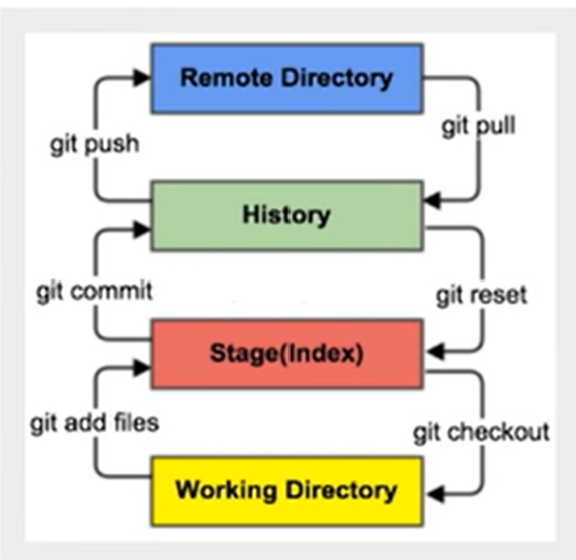
\includegraphics{gitfigure}
\end{center}

\begin{center}
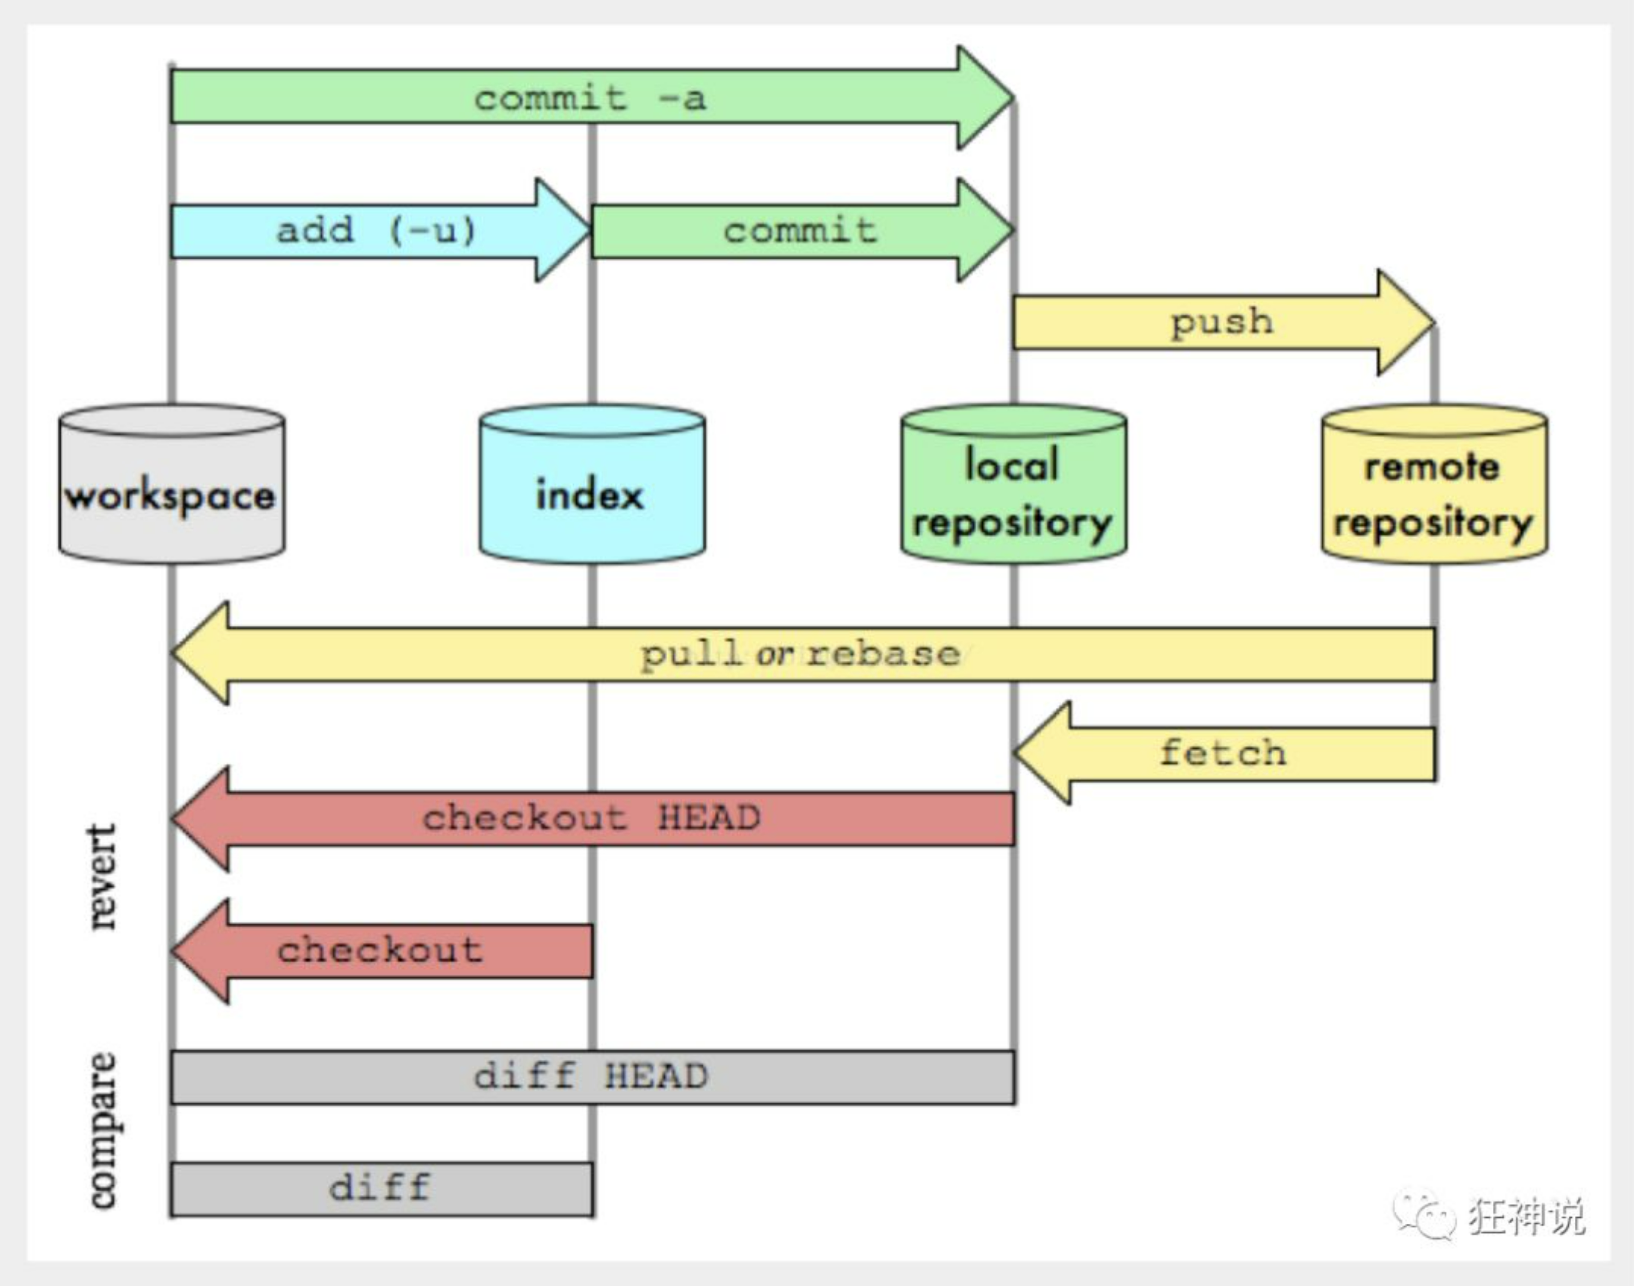
\includegraphics[scale=0.6]{666}
\end{center}

First of all, open Git Bash by right clicking at the directory where you want to work with. 

You can also input 
\begin{verbatim}
cd your_folder_name
\end{verbatim}
to change your path. 

Then input 
\begin{verbatim}
git clone github_code_link
\end{verbatim}
 to clone that repository. 

\textit{In order to get the code link, you go to a github repository and click the green button \textbf{Code}, then copy the HTTPS link. }

\section{Editing, add and commit}
After editing your files in your computer, you can input \begin{verbatim}
git add file_name or git add --all \end{verbatim}, then input \begin{verbatim}
git status \end{verbatim} to check which step are you now, "lets you inspect the working directory and the staging area", then input \begin{verbatim} git commit -m"editing message" \end{verbatim}, and now input \begin{verbatim} git push \end{verbatim} to ensure your change is uploaded to github

\textbf{note that, when adding a folder, that folder must have some contents}
\begin{verbatim}
git add folder_name
\end{verbatim}

\section{Advanced usage}
\subsection{Upload what you have created}
To create a directory at your computer, do as following:  \begin{verbatim}
cd folder_name

git config --global user.name "your name"

git config --global user.email your_e-mail

git init
\end{verbatim}
This will set the author to be your name. "You’ll typically only need to use this immediately after installing Git on a new development machine."

\textbf{optional to create a file:}
\begin{verbatim}
echo "file content" > file_name.file_type
touch file_name.file_type
\end{verbatim}

\begin{verbatim}
git log 
\end{verbatim} to see all versions, press q to quit, "only operates on the committed history." 

To ignore some files:
\begin{verbatim}
touch .gitignore
\end{verbatim}, and then input the file name in the .gitignore file

To add an new branch
\begin{verbatim}
git branch branch_name
git checkout branch_name  -->to switch to new branch
git commit -a -m"comments"  -->to add and commit simultaneously, 
but note that for untracked files, -a does not work
git branch -d branch_name -->delete a branch
git branch -D_branchname -->delete a branch definitly
git checkout -b branch_name -->create and go to an new branch
git merge other_branch -->merge other branch to present branch
\end{verbatim}

\subsection{Download from github repository}

\begin{verbatim}
git remote -v -->to see what relation is there from your PC and github repository
git fetch 
git diff repository_name/branch_name
git pull 
\end{verbatim}

\textbf{\textit{The pull command only download what changed in repository, and will not cover what file or content you have added in your directory. }}

\subsection{git reset to go back to previous version}

\begin{center}
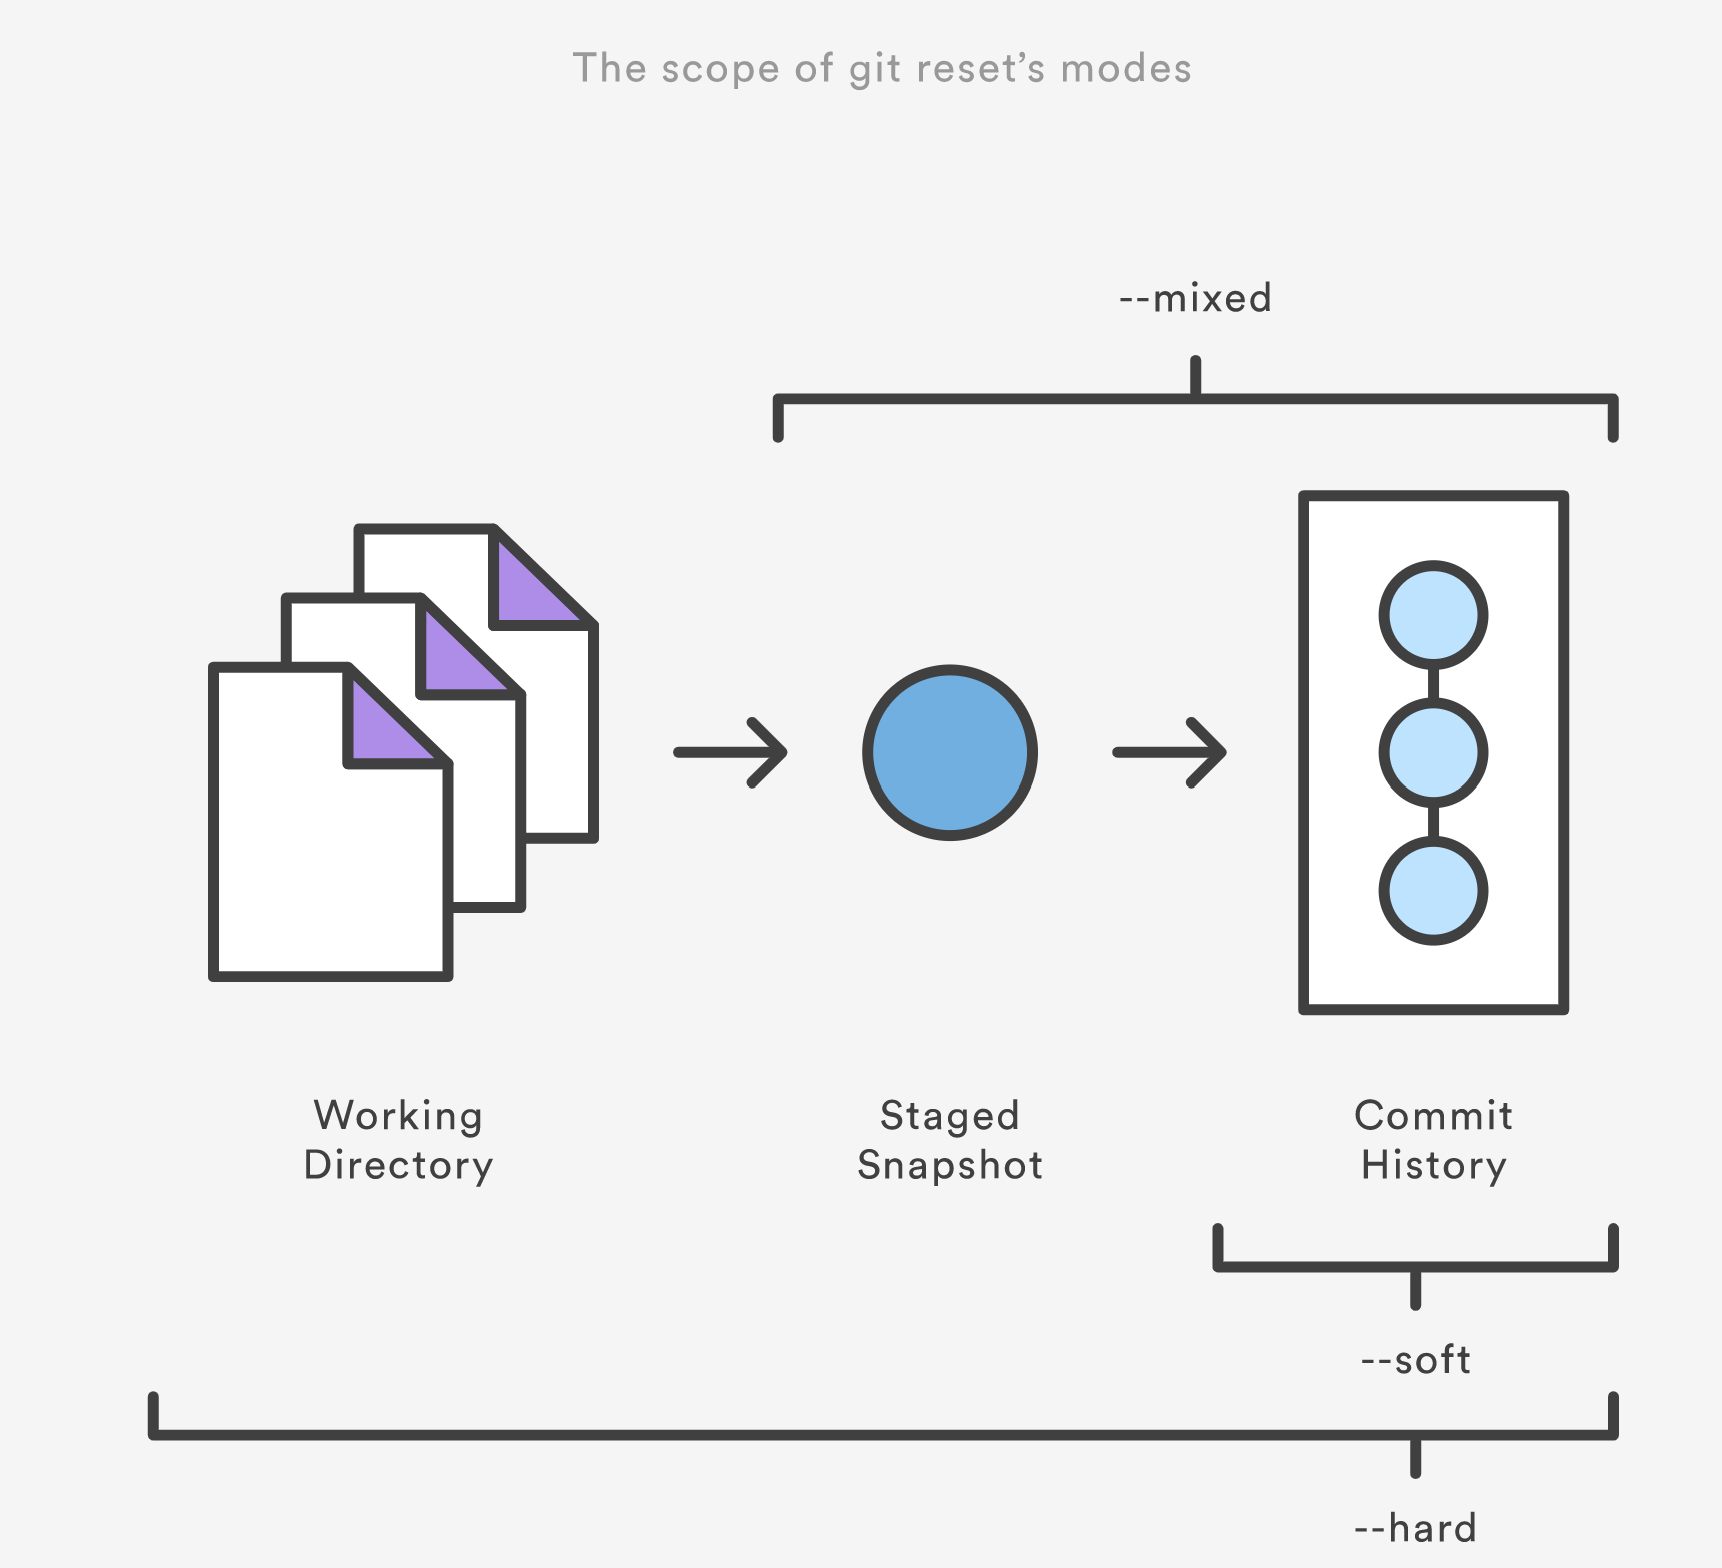
\includegraphics[scale=0.3]{gitreset}
\end{center}

\begin{verbatim}
git reset 
\end{verbatim}
has 3 options, --mixed, --soft and --hard, --mixed is the default option. 

\subsection{Some Linux command}
\begin{verbatim}
cd --> change directory
cd.. -->go back to last directory
pwd --> show present path
ls --> listing all documents in present directory
touch name.file_form  --> create a new file 
rm file_name --> remove/delete that file
mkdir --> create a new directory/folder

DO NOT RUN THIS: rm -rf --> delete all files in this computer

mv this.file this.folder --> move a file to a folder,
 the file and the folder should be in the same directory
clear --> clean the screen
\end{verbatim}



\section{Reference}
\begin{verbatim}
Chinese Only
https://mp.weixin.qq.com/s/Bf7uVhGiu47uOELjmC5uXQ 

Chinese Only
https://www.bilibili.com/video/BV1r3411F7kn/

English
https://www.atlassian.com/git/glossary 
\end{verbatim}

\end{document}